\documentclass[letterpaper,10pt, jcp, aps]{revtex4-1}

\usepackage[utf8]{inputenc}
\usepackage[spanish]{babel}
\usepackage{amsmath, amsfonts}
\usepackage{graphicx}
\usepackage{natbib}
\usepackage{caption}
\usepackage{subcaption}
%\usepackage{authblk} parece ser que ya esta metido cuando usas preprint


%\bibliographystyle{alpha}

%opening

%\author{Rosa Rodríguez \& David P.~Sanders \& W. P. K. Zapfe}
%\affil{Departamento de Física, Facultad de Ciencias, Universidad Nacional Autónoma de México, Ciudad Universitaria, Del.~Coyoacán, México D.F. 04510, Mexico}

\usepackage{mathptmx}
% I dont know if that package is compatible with revtex.

\newcommand{\defeq}{:=}
\newcommand{\mean}[1]{\left \langle #1 \right \rangle}
\newcommand{\rd}{\!\mathrm{d}}
\newcommand{\RR}{\mathbb{R}}
\newcommand{\vv}{\mathbf{v}}
\newcommand{\indicator}[1]{\mathbf{1}_{ \{   #1 \} } } 
\newcommand{\etal}{\emph{et al.\ }} 

\setlength{\parskip}{10pt}
\setlength{\parindent}{0pt}


\begin{document}

\title{Una extraña raiz de tres y un cambio cualitativo en el comportamiento}

\section{maldita raiz de tres}

Okey David, si las cuentas están bien, el factor constante en la fórmula de
Machta-Zwanzig debería de ser:
\begin{equation} \label{meantimegeneralredux}
   \frac{1}{\sqrt{2E / m}} 
\frac{|S^3|}{|B^3|}=\frac{3\pi}{2\sqrt{2}},	 
\end{equation}
Si usamos $E=1, m=1$


He checado que el volumen del paralelipedido cuadridimensional y el área de
``hopping cross section'' estuviera bien numéricamente, y ambas le pegan
muy bien a lo obtenido de las integrales analíticas. Así que ahí no tengo error alguno.
Pero cuando aplico la fórmula de MZ al hopping obtengo algo muy raro:
La función parece estar multiplicada por EXACTAMENTE $\sqrt{3}$. En el caso
de $w=1.5,h=1$ me sale lo que muestro en la figura \ref{w75h50}.
En algun momento pensé que se debería a algo raro en el volumen de la mesa,
dado que tiene una relación de aspecto de 3/2, y que tal vez de ahí provendría
el error, pero no: luego revise con varias proporciones, y siempre da lo mismo, como
te mostraré en la próxima sección. La numérica esta un poco baja ahorita porque
me desesperaba hacer varias pruebas rápido, pero creo que es aceptablemente buena
para mostrarte mi punto. Hay una desviación de una pancita por ahí, voy a checar que es.


\begin{figure}[h]
\centering
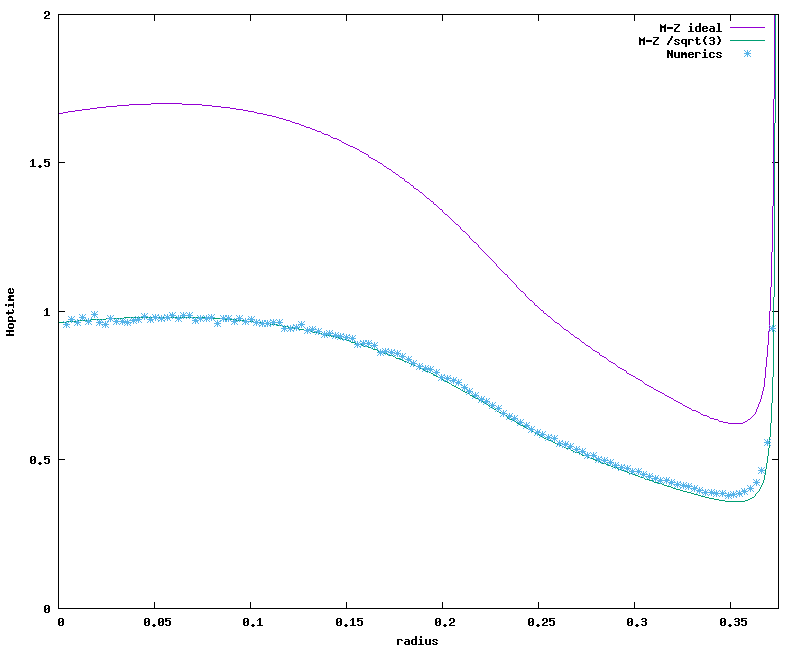
\includegraphics[width=0.45\textwidth]{./FigurasPerfectas/Hopw75h50-01.png}\caption{El tiempo promedio de ``hopping'' vertical, analítico, numérico, y analítico
divido por $\sqrt{3}$.}  
}\label{w75h50} 
\end{figure}


\section{Cambio cualitativo de comportamiento.}

Okey David, ¿te acuerdas de que cuando trabajabamos la mesa cuadrada
esperabamos que conforme el radio fuera al límite permisible los brincos fueran
mas y mas raros, hasta que fueran imposibles y el tiempo decreciera?
Pues eso es falso en general. Resulta que en casos más generales, donde puedes acomodar los discos mas gordos de forma que sigan pasando unos junto a otros pero que tengas poco
lugar donde acomodarlos, el tiempo de ``hopp'' decrece. Porque en realidad
lo que pasa es que no tienen mucho hacia donde ir: cuando ya no pueden hacer hop horizontal pero todavía pueden hacerlo vertical, lo hacen. La figura de arriba muestre ese comportamiento, observa como hay dos puntos críticos en la función, antes de que se vuelva
super dificil hacer que un disco pase uno junto al otro, hay un momento en que son muy grandes pero rebotan muy seguido entre arriba y abajo (y ya no pueden intercambiar de sitio horizontal, dado que h=1.0, el radio máximo donde podrían hacerlo es 0.25... ¿¿¿ahí esta
el punto de inflección???). Observa la siguiente tabla de figuras (en todas la
función analítica aparece divida por el misterioso $\sqrt{3}$). 



    \begin{figure}
    \centering
    \begin{subfigure}[b]{0.35\textwidth}
        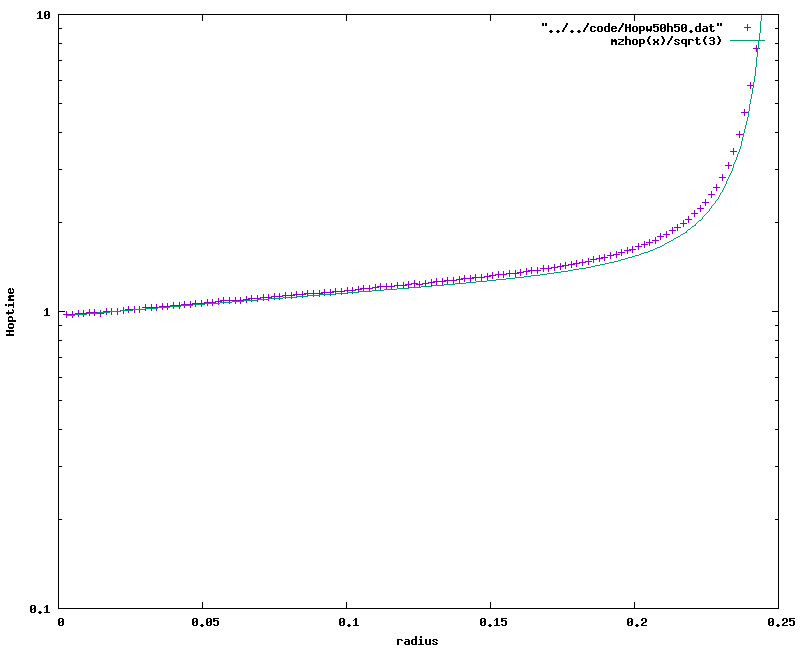
\includegraphics[width=\textwidth]{FigurasPerfectas/Hopw50h50-01.png}
        \caption{w/h=1}
        \label{wh1}
    \end{subfigure}
    ~ %add desired spacing between images, e. g. ~, \quad, \qquad, \hfill etc. 
      %(or a blank line to force the subfigure onto a new line)
    \begin{subfigure}[b]{0.35\textwidth}
        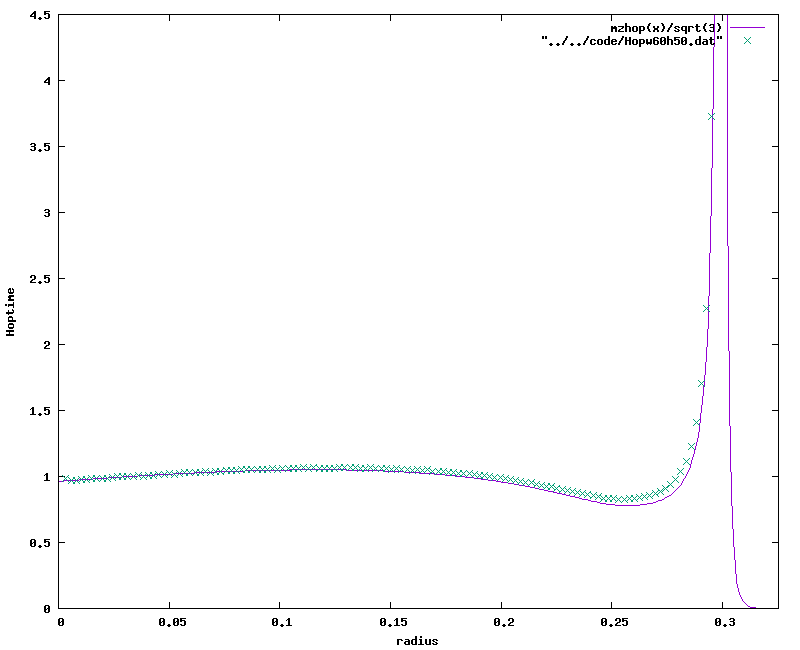
\includegraphics[width=\textwidth]{FigurasPerfectas/Hopw60h50.png}
        \caption{w/h=1.2}
        \label{wh12}
    \end{subfigure}
    \\
    \begin{subfigure}[b]{0.35\textwidth}
        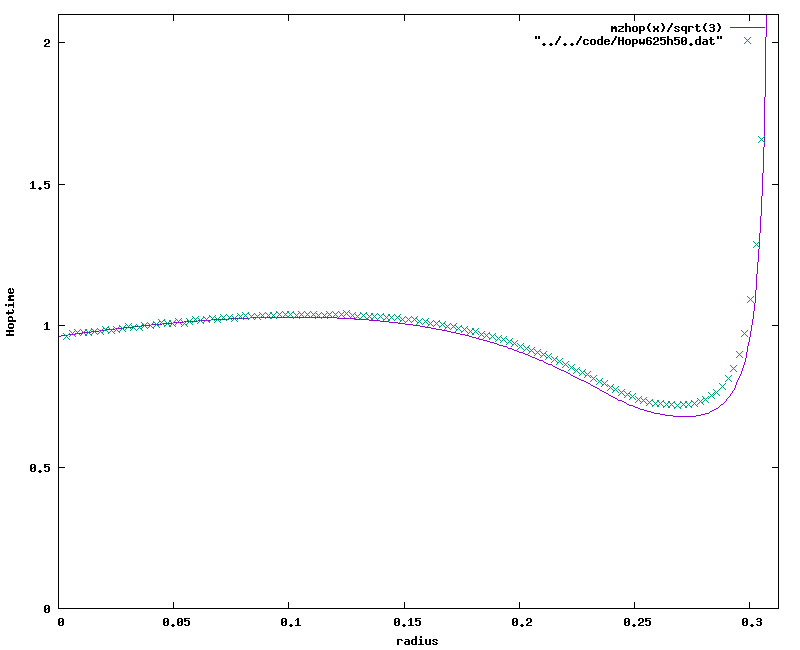
\includegraphics[width=\textwidth]{FigurasPerfectas/Hopw625h50.png}
        \caption{w/h=1.25}
        \label{wh125}
    \end{subfigure}
    ~ %add desired spacing between images, e. g. ~, \quad, \qquad, \hfill etc. 
      %(or a blank line to force the subfigure onto a new line)
    \begin{subfigure}[b]{0.35\textwidth}
        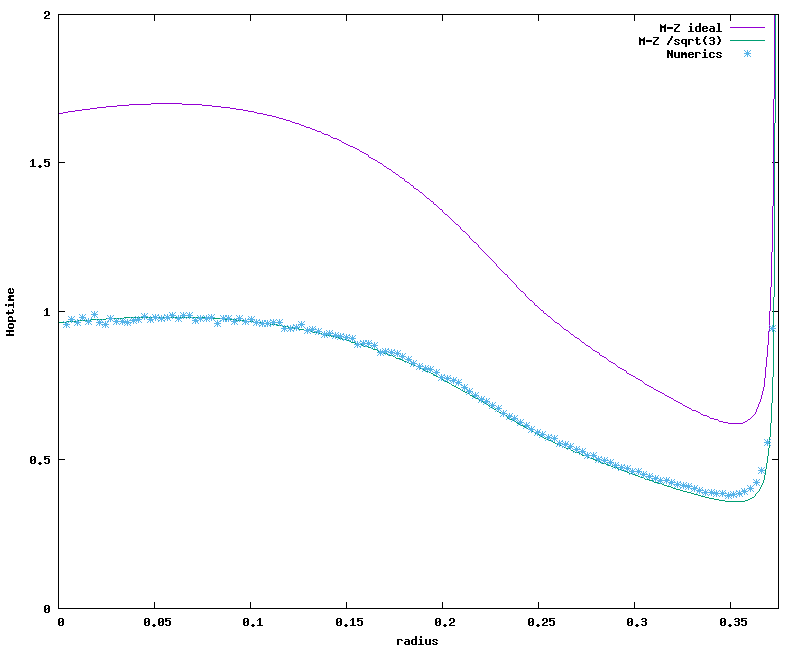
\includegraphics[width=\textwidth]{FigurasPerfectas/Hopw75h50-01.png}
        \caption{w/h=1.5}
        \label{wh15}
    \end{subfigure}
    \\
      \begin{subfigure}[b]{0.35\textwidth}
        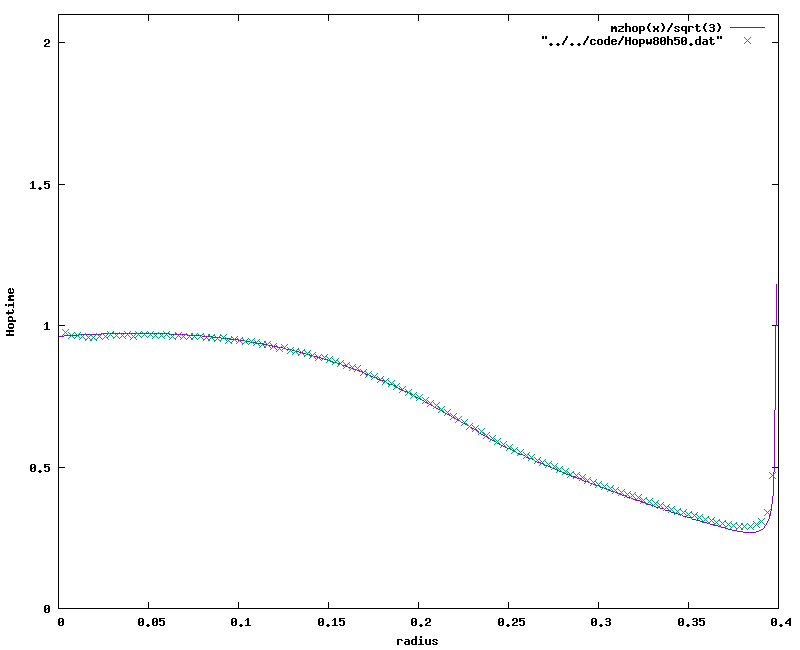
\includegraphics[width=\textwidth]{FigurasPerfectas/Hopw80h50.png}
        \caption{w/h=1.6}
        \label{wh16}
    \end{subfigure}
    ~ %add desired spacing between images, e. g. ~, \quad, \qquad, \hfill etc. 
      %(or a blank line to force the subfigure onto a new line)
    \begin{subfigure}[b]{0.35\textwidth}
        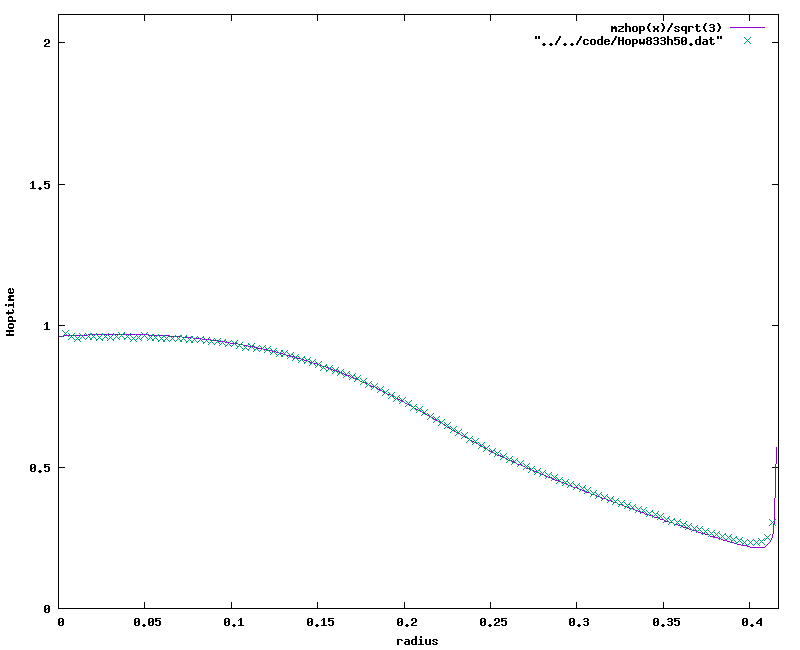
\includegraphics[width=\textwidth]{FigurasPerfectas/Hopw833h50.png}
        \caption{w/h=5/3}
        \label{wh53}
    \end{subfigure}
    \\
      \begin{subfigure}[b]{0.35\textwidth}
        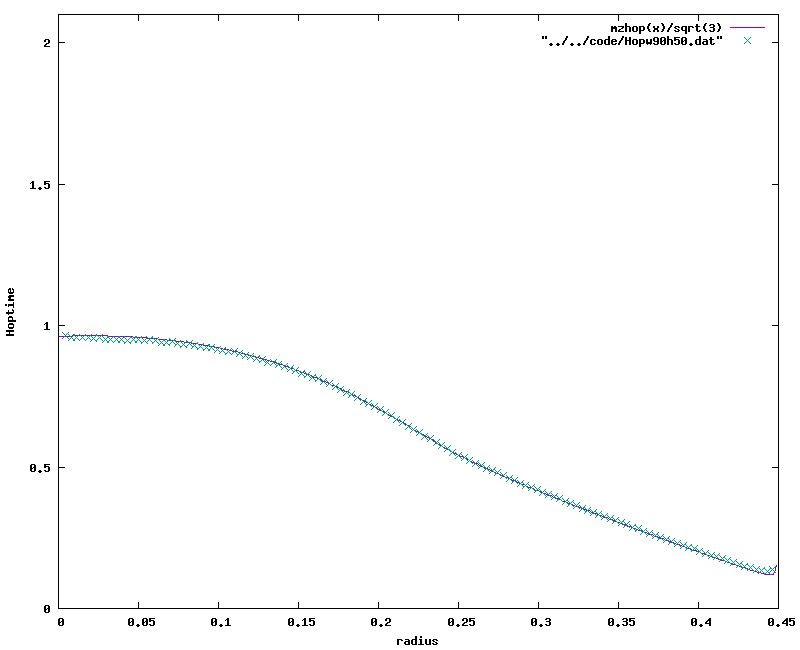
\includegraphics[width=\textwidth]{FigurasPerfectas/Hopw90h50.png}
        \caption{w/h=1.8}
        \label{wh1}
    \end{subfigure}
    ~ %add desired spacing between images, e. g. ~, \quad, \qquad, \hfill etc. 
      %(or a blank line to force the subfigure onto a new line)
    \begin{subfigure}[b]{0.35\textwidth}
        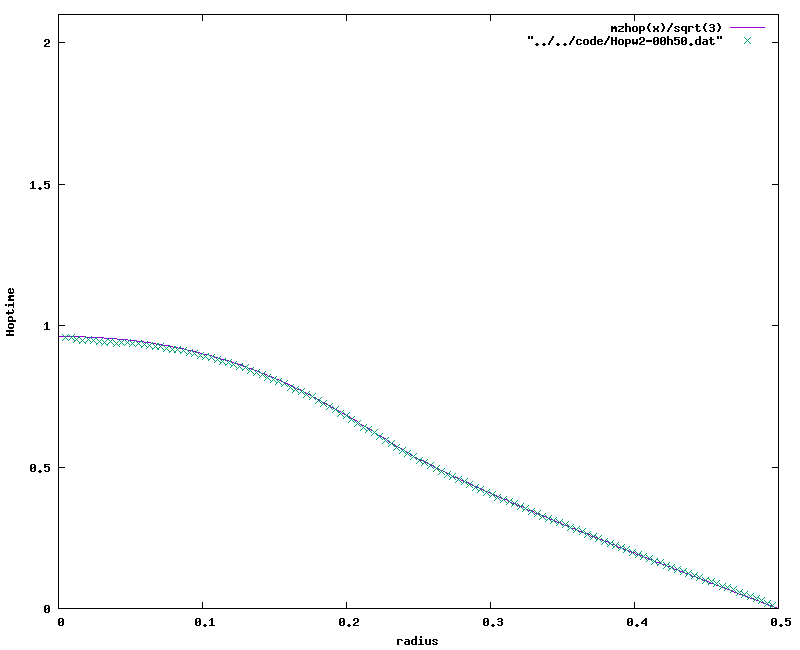
\includegraphics[width=\textwidth]{FigurasPerfectas/Hopw2-00h50.png}
        \caption{w/h=2.0}
        \label{wh18}
    \end{subfigure}
    \caption{Pictures of animals}\label{fig:animals}
\end{figure}













\end{document}
